\documentclass[../Main.tex]{subfiles} 
\begin{document}

\section{Algorithms}
Unsere grundlegende Datenstruktur sind Vektoren, deren Stellen die Regionen repräsentieren. Für unsere Arbeit mit sieben festgelegten Regionen kommen also siebenstellige Vektoren zum Einsatz.
Vektoren werden bei uns einerseits Wörtern (Types) und andererseits Tweets (Dokumenten) zugeordnet. Sie zeigen jeweils die Stärke der Zugehörigkeit des Wortes beziehungsweise des Tweets zu den einzelnen Regionen.

So könnte zum Beispiel das Wort \glqq Porree\grqq{} zu je einem Drittel signifikant für die Regionen Ostdeutschland, Norddeutschland und Westdeutschland sein. Damit würde man die Wahrscheinlichkeit, dass eine Benutzung dieses Wortes auf einen Sprecher aus einer dieser Regionen hinweist, auf jeweils ein Drittel schätzen, für die anderen Regionen jeweils auf Null.

$$\overrightarrow{Porree} = \begin{pmatrix} 0,33 \\ 0,33 \\ 0,33 \\ 0,0 \\ 0,0 \\ 0,0 \\ 0,0 \end{pmatrix} \ \ \ \ \begin{matrix} \text{Ostdeutschland} \\ \text{Norddeutschland} \\ \text{Westdeutschland} \\ \text{Bayern} \\ \text{Südwestdeutschland} \\ \text{Österreich} \\ \text{Schweiz} \end{matrix}$$

Als Saat werden initiale Wortvektoren \textit{(0. Generation)} verwendet. Besonders beim Regiowort-Ansatz handelt es sich hier um eine sehr geringe Menge, die noch nicht zur Anwendung taugt -- es gäbe in einem zu klassifizierenden Tweet schlicht nur mit geringster Wahrscheinlichkeit überhaupt einen Treffer.

Daher folgt nun eine Anreicherungsphase, in der mithilfe von Twitter-Trainingsdaten weitere regional signifikante Wörter gefunden werden sollen. Dies erledigt unser Haupt-Algorithmus, der aus einer Generation von Wortvektoren die nächste Generation berechnet. Er kann also in einer Schleife mit beliebiger Anzahl von Durchläufen angewendet werden. Schließlich liegt eine finale Generation von Wortvektoren vor. Daraus berechnen wir noch den Durchschnittsvektor (normalisiert auf Länge 1), dann ist unser Modell fertig trainiert.

In der Anwendung wird nun zu einem ungesehenen Tweet ein Tweetvektor berechnet. Dazu wird er nach Wörtern durchsucht, zu denen Wortvektoren vorliegen. Alle Wortvektoren zu gefundenen Wörtern werden dann aufsummiert.
Anschließend wird der Tweetvektor auf Länge 1 normalisiert. Zur Zuordnung des Tweets zu einer Region wird nun die Differenz aus dem Durchschnittsvektor und dem Tweetvektor berechnet. Das Ergebnis ist ein Differenzvektor, der in die gesuchte Richtung weist. Genauer gesagt verrät der größte Wert dieses Vektors, in Richtung welcher Region der Vektor am stärksten zeigt. Diese Region ist das Ergebnis unserer Klassifikation.

\subsection{Main algorithm}
Der Haupt-Algorithmus erzeugt aus einer bestehenden Generation von Wortvektoren und einem Trainingskorpus mit Tweets eine neue Generation von Wortvektoren.

Es wird über alle Tweets im Trainingskorpus iteriert. Für jeden Tweet wird zunächst ein Tweetvektor berechnet. Dazu wird einfach zu jedem Token des Tweets der Wortvektor der bestehenden Generation -- sofern er existiert -- aufsummiert. Anschließend wird umgekehrt für jedes Token des Tweets der Tweetvektor zum neuen Wortvektor addiert. Falls einige Token des Tweets in der alten Generation von Wortvektoren nicht vertreten sind, so kommen sie in der neuen Generation nun neu hinzu; die Zahl der Wortvektoren erhöht sich also. Es verändern sich aber auch die Werte für die bereits vorhandenen Wörter.

Zusammengefasst wird also erst für jeden Tweet des Trainingskorpus ein Tweetvektor auf Basis der bestehenden Wortvektoren zu den darin vorkommenden Wörtern berechnet, und anschließend für jedes Wort im Trainingskorpus ein Wortvektor auf Basis der Tweetvektoren zu den Tweets, in denen es vorkommt.

\begin{algorithm}[H]
 \SetAlgoLined
 \KwData{\\
	$WV_0$: bestehende Menge von Wortvektoren $WV_0(Wort) = \vec V_{Wort}$\\ 
	$Tweets$: Menge von Tweets\\ $ $}
 \KwResult{\\$WV_1$: angereicherte Menge von Wortvektoren $WV_1(Wort) = \vec V_{Wort}$\\ $ $}
 $WV_1 \gets\emptyset $\; 
\ForEach{Tweet in Tweets}{
 $\vec V_{Tweet} \gets (0,0,0,0,0,0,0)$\\
 \ForAll{Token in Tweet}{
  $\vec V_{Tweet}  \gets \vec V_{Tweet} + WV_0(Token)$
}
 \ForAll{Token in Tweet}{
  $WV_1(Token)  \gets WV_1(Token) + \vec V_{Tweet}$
}
}
 \ForEach{$\vec V_{Word}$ in $WV_1$}{
$\vec V_{Word}$ $\gets$ normalize($\vec V_{Word}$)
}
\Return $WV_1$\;
\caption{Tweegion Main-Algorithm}
\end{algorithm}

% \subsection{Difference between both attempts}
\subsection{Normalizing versions}
Im Laufe der Arbeit haben wir mehrere Varianten unseres Haupt-Algorithmus entwickelt, die sich in der Behandlung der Wortvektoren nach jedem Durchlauf, also im Anschluss an die Berechnung der Tweet- und der Wortvektoren, unterscheiden. Diese Behandlung wirkt sich direkt auf die folgende Berechnung von Tweetvektoren aus, sowohl in einem möglichen folgenden Durchlauf des Haupt-Algorithmus wie auch bei der Anwendung, also der Klassifizierung eines ungesehenen Tweets.

Die ursprüngliche Version, \textit{Normalized,} sieht eine Normalisierung aller Wortvektoren jeweils auf Summe 1 vor. Das bedeutet, dass jedes Type gleichwertig ist, unabhängig von der Anzahl der Token. Bei Testläufen sahen wir, dass dieses Vorgehen seltene Wörter extrem bevorzugt, da diese nur in einem oder wenigen Tweets vorkommen und damit sehr stark regional gewertet werden.

Unsere zweite Variante, \textit{Linear,} entstand dann einfach durch das Auslassen der Normalisierung. Hier besitzt nun jedes Type ein Gewicht in direkter linearer Abhängigkeit seiner Häufigkeit als Token. Diese Variante, so zeigte sich, verlieh aber sehr häufigen Wörtern ein so großes Gewicht, dass die regionale Signifikanz, die sich eher bei Wörtern mit mittlerer Häufigkeit findet, stark einbüßte und es nur noch winzige Abweichungen vom Durchschnittsvektor gab.

Auf Grundlage dieser Erfahrungen beschlossen wir, einen Kompromiss zwischen konstanter und linearer Abhängigkeit zu finden. Wir entwickelten also die Variante \textit{Log,} bei der die Länge des Vektors so verändert wird, dass dabei die Summe des Vektors erhöht um 1 zur Basis 2 logarithmiert wird.

$$\vec v = \frac{\vec v}{\sum_i v_i} * \log_2(\sum_i v_i+1)$$

Bei der Variante \textit{Root} wird hier statt dem Logarithmus zur Basis 2 die Quadratwurzel genutzt.

$$\vec v = \frac{\vec v}{\sum_i v_i} * \sqrt{\sum_i v_i}$$

\subsection{Cosine similarity}
\begin{figure}
  \[ sim(\vec{q},\vec{d_j}) = \frac{\sum^N_{i=1} w_{i,q} \times w_{i,j}}{\sqrt{\sum^N_{i=1}w^2_{i,q}} \times \sqrt{\sum^N_{i=1}w^2_{i,j}}} \]
  \caption{Cosine similarity}
  \label{cos_sim}
\end{figure}
\begin{figure}
 \begin{align*}
  q &= \textrm{'Ich glaube @Drahflow tippt noch schneller als er redet. ;) \#om13' } \\
  \vec{q} &= (0.427, 0.38, 0.4, 0.39, 0.391, 0.602,  0.41) \\ 
   \vec{\bar{d}} &= \frac{\sum^N_{i=0} d_i}{N} =  (0.376, 0.336, 0.349, 0.346, 0.361, 0.481,  0.379) \\
  sim(\vec{q}, \vec{\bar{d}}) &= 0.9986 
\end{align*}
  \caption{Example for the similarity calculation}
  \label{cos_sim_example}
\end{figure}
Although Tweets may differ from one region to another in some way, a huge percentage of the German Twitter users write their messages exclusively in standard German with no signs of any regional influence whatsoever.  \\
For example the following Tweet just appeared in my timeline:
\begin{quote}
'Ich glaube @Drahflow tippt noch schneller als er redet. ;) \#om13'
\end{quote}
Keeping in mind that  usernames, hashtags, smileys and punctation are being removed in the pre-processing, this Tweet contains way to ordinary words to be assigned to a specific region. It is written in pure High German and therefore could be sent from a town in Bavaria as well as from Berlin and depending on the data we use to train our algorithm with, the result of the program could be 'Austria' or 'Northern Germany' as well.

To face this problem we decided to filter this kind of undistinguished Tweets to have more reliable results and because of that also increase the accuracy of the algorithm. \\
Our idea was to determine the average Tweet-vector $\vec{\bar{d}}$ of all the Tweets in the training-corpus and to compare the Tweet-vector $\vec{q}$ of a given Tweet with it, using the cosine metric (see Figure \ref{cos_sim} on page \pageref{cos_sim}) as recommended  in Jurafsky \& Martin. If the similarity between both vectors is smaller than a specified threshold, we continue to map the Tweet to one of the region, if not we stop and return a message, that the Tweet is written in standard German and can not be classified. In the example in figure \ref{cos_sim_example} on page \pageref{cos_sim_example}, the vector $\vec{q}$ for the Tweet mentioned above is compared to the average Tweet-vector $\vec{\bar{d}}$, returning a very high similarity of $0.9986$. Nevertheless the algorithm states, that the Tweet was most likely sent from Switzerland. 

But the most difficult thing was to find the right threshold, that separates the too ordinary Tweets from the regional ones. To make a guess which percentage of all Tweets are written in standard German, we calculated the cosine similarity of all Tweets in the training-corpus to the average vector, sorted them and had a look at the distribution (figure \ref{cos_distribution} in page \pageref{cos_distribution}). \\
The result was not surprising: More than 80\% of all Tweets had a similarity of 0.9 or higher. Or, seen from another point of view, only 20\% of all Tweets differ enough from the average vector to calculate reliable results. 

In the experiments in the sections 3 (regional based attempt) and 4 (geo location based) we tested different thresholds to find a good balance between a reliable classification with a high accuracy and the coverage of as many Tweets as possible.

\begin{figure}
  \begin{center}
   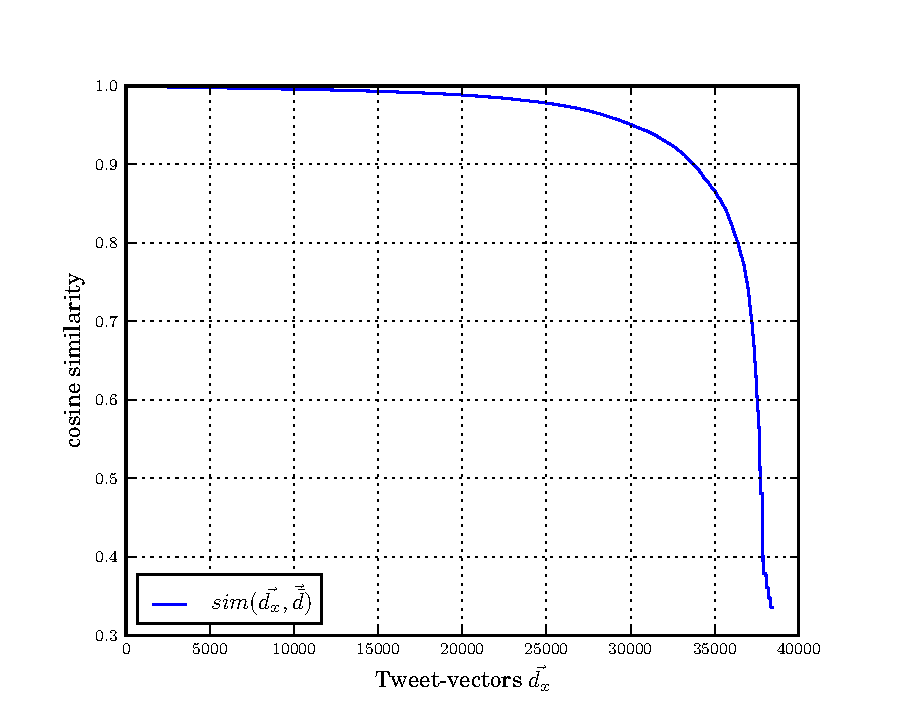
\includegraphics[width=\columnwidth]{../img/cos-verteilung.eps}
    \caption{\label{cos_distribution} Cosine similarity between all Tweet-vectors and the average Tweet-vector}
  \end{center}
\end{figure}

% \subsection{Evaluation}

\end{document}
